\section{\ac{SAT}-solvers}

SMT vs. SAT is like high level \ac{PL} vs. assembly language.
The latter can be much more efficient, but it's hard to program in it.

\subsection{CNF form}

\ac{CNF}\footnote{\url{https://en.wikipedia.org/wiki/Conjunctive_normal_form}} is a \textit{normal form}.

% TODO recheck
% TODO write abt it!
%\textit{normal form} is somewhat similar to polynomials in algebra. 
%What is polynomial?
%It is a standard way to express unsystematic equations like $2x \cdot x$ as $3x$ polynomial, 
%and so you will be able to apply some operations to polynomials like summing, etc.

Any boolean expression can be converted to \textit{normal form} and \ac{CNF} is one of them.
The \ac{CNF} expression is a bunch of clauses (sub-expressions) constisting of terms (variables), ORs and NOTs, 
all of which are then glueled together with AND into a full expression.
There is a way to memorize it: \ac{CNF} is ``AND of ORs'' (or ``product of sums'') and \ac{DNF} is ``OR of ANDs'' (or ``sum of products'').

Example is: $(\neg A \vee B) \wedge (C \vee \neg D)$.

$\vee$ stands for OR (logical disjunction\footnote{\url{https://en.wikipedia.org/wiki/Logical_disjunction}}), 
``+'' sign is also sometimes used for OR.

$\wedge$ stands for AND (logical conjunction\footnote{\url{https://en.wikipedia.org/wiki/Logical_conjunction}}).
It is easy to memorize: $\wedge$ looks like ``A'' letter.
``$\cdot$'' is also sometimes used for AND.

$\neg$ is negation (NOT).

% TODO A/B is the first clause, C/D is second

\subsection{Example: 2-bit adder}
\label{adder}

\ac{SAT}-solver is merely a solver of huge boolean equations in CNF form.
It just gives the answer, if there is a set of input values which can satisfy CNF expression, and what input values must be.

Here is a 2-bit adder for example:

\begin{figure}[ht!]
\centering
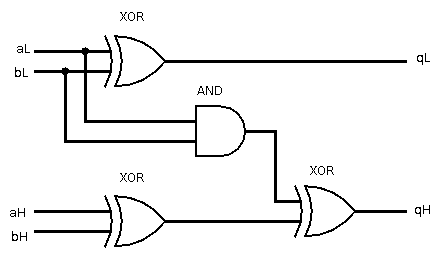
\includegraphics[scale=0.75]{SAT/adder_logisim.png}
\caption{2-bit adder circuit}
\end{figure}

The adder in its simplest form: it has no carry-in and carry-out, and it has 3 XOR gates and one AND gate.
Let's try to figure out, which sets of input values will force adder to set both two output bits?
By doing quick memory calculation, we can see that there are 4 ways to do so: $0+3=3$, $1+2=3$, $2+1=3$, $3+0=3$.
Here is also truth table, with these rows highlighted:

\newcommand{\HLcell}{\cellcolor{blue!25}}

\begin{center}
\begin{doublespace}
\noindent\(\begin{array}{l|llllll}
  & \text{aH} & \text{aL} & \text{bH} & \text{bL} & \text{qH} & \text{qL} \\
\hline
 \text{3+3 = 6 $\equiv $ 2 (mod 4)} & 1 & 1 & 1 & 1 & 1 & 0 \\
 \text{3+2 = 5 $\equiv $ 1 (mod 4)} & 1 & 1 & 1 & 0 & 0 & 1 \\
 \text{3+1 = 4 $\equiv $ 0 (mod 4)} & 1 & 1 & 0 & 1 & 0 & 0 \\
 \text{\HLcell{}3+0 = 3 $\equiv $ 3 (mod 4)} & \HLcell{}1 & \HLcell{}1 & \HLcell{}0 & \HLcell{}0 & \HLcell{}1 & \HLcell{}1 \\
 \text{2+3 = 5 $\equiv $ 1 (mod 4)} & 1 & 0 & 1 & 1 & 0 & 1 \\
 \text{2+2 = 4 $\equiv $ 0 (mod 4)} & 1 & 0 & 1 & 0 & 0 & 0 \\
 \text{\HLcell{}2+1 = 3 $\equiv $ 3 (mod 4)} & \HLcell{}1 & \HLcell{}0 & \HLcell{}0 & \HLcell{}1 & \HLcell{}1 & \HLcell{}1 \\
 \text{2+0 = 2 $\equiv $ 2 (mod 4)} & 1 & 0 & 0 & 0 & 1 & 0 \\
 \text{1+3 = 4 $\equiv $ 0 (mod 4)} & 0 & 1 & 1 & 1 & 0 & 0 \\
 \text{\HLcell{}1+2 = 3 $\equiv $ 3 (mod 4)} & \HLcell{}0 & \HLcell{}1 & \HLcell{}1 & \HLcell{}0 & \HLcell{}1 & \HLcell{}1 \\
 \text{1+1 = 2 $\equiv $ 2 (mod 4)} & 0 & 1 & 0 & 1 & 1 & 0 \\
 \text{1+0 = 1 $\equiv $ 1 (mod 4)} & 0 & 1 & 0 & 0 & 0 & 1 \\
 \text{\HLcell{}0+3 = 3 $\equiv $ 3 (mod 4)} & \HLcell{}0 & \HLcell{}0 & \HLcell{}1 & \HLcell{}1 & \HLcell{}1 & \HLcell{}1 \\
 \text{0+2 = 2 $\equiv $ 2 (mod 4)} & 0 & 0 & 1 & 0 & 1 & 0 \\
 \text{0+1 = 1 $\equiv $ 1 (mod 4)} & 0 & 0 & 0 & 1 & 0 & 1 \\
 \text{0+0 = 0 $\equiv $ 0 (mod 4)} & 0 & 0 & 0 & 0 & 0 & 0 \\
\end{array}\)
\end{doublespace}
\end{center}


Let's find, what \ac{SAT}-solver can say about it?

First, we should represent our 2-bit adder as \ac{CNF} expression.

Using Wolfram Mathematica, we can express 1-bit expression for both adder outputs:\\
\\
\textbf{\texttt{In[]:=AdderQ0[aL$\_$,bL$\_$]=Xor[aL,bL]}} \\
\textbf{\texttt{Out[]:=aL $\veebar$ bL}} \\
\\
\textbf{\texttt{In[]:=AdderQ1[aL$\_$,aH$\_$,bL$\_$,bH$\_$]=Xor[And[aL,bL],Xor[aH,bH]]}} \\
\textbf{\texttt{Out[]:=aH $\veebar$ bH $\veebar$ (aL \&\& bL)}} \\
\\
We need such expression, where both parts will generate 1's.
Let's use Wolfram Mathematica find all instances of such expression (I glueled both parts with And): \\
\\
\textbf{\texttt{In[]:=Boole[SatisfiabilityInstances[And[AdderQ0[aL,bL],AdderQ1[aL,aH,bL,bH]],\{aL,aH,bL,bH\},4]]}} \\
\textbf{\texttt{Out[]:=\{1,1,0,0\},\{1,0,0,1\},\{0,1,1,0\},\{0,0,1,1\}}} \\
\\
Yes, indeed, Mathematica says, there are 4 inputs which will lead to the result we need.
So, Mathematica can also be used as \ac{SAT} solver.

Nevertheless, let's proceed to \ac{CNF} form. Using Mathematica again, let's convert our expression to \ac{CNF} form:\\
\\
\textbf{\texttt{In[]:=cnf=BooleanConvert[And[AdderQ0[aL,bL],AdderQ1[aL,aH,bL,bH]],``CNF'']}} \\
\textbf{\texttt{Out[]:=(!aH $\|$ !bH) \&\& (aH $\|$ bH) \&\& (!aL $\|$ !bL) \&\& (aL $\|$ bL)}} \\
\\
Looks more complex. The reason of such verbosity is that \ac{CNF} form doesn't allow XOR operations.
% FIXME: TeX form of the expression!

\subsubsection{MiniSat}

For starters, we can try MiniSat\footnote{\url{http://minisat.se/MiniSat.html}}.
The standard way to encode \ac{CNF} expression for MiniSat is to enumerate all OR parts at each line.
Also, MiniSat doesn't support variable names, just numbers.
Let's enumerate our variables: 1 will be aH, 2 -- aL, 3 -- bH, 4 -- bL.

Here is what I've got when I converted Mathematica expression to the MiniSat input file:

\lstinputlisting{SAT/adder.cnf}

Two 4's at the first lines are number of variables and number of clauses respectively.
There are 4 lines then, each for each OR clause.
Minus before variable number meaning that the variable is negated.
Absence of minus -- not negated.
Zero at the end is just terminating zero, meaning end of the clause.

In other words, each line is OR-clause with optional negations,
and the task of MiniSat is to find such set of input, which can satisfy all lines in the input file.

That file I named as \textit{adder.cnf} and now let's try MiniSat:

\begin{lstlisting}
% minisat -verb=0 adder.cnf results.txt
SATISFIABLE
\end{lstlisting}

The results are in \textit{results.txt} file:

\begin{lstlisting}
SAT
-1 -2 3 4 0
\end{lstlisting}

This means, if the first two variables (aH and aL) will be \textit{false}, and the last two variables (bH and bL) will be set to \textit{true},
the whole \ac{CNF} expression is satisfiable.
Seems to be true: if bH and bL are the only inputs set to \textit{true}, both resulting bits are also has \textit{true} states.

Now how to get other instances? \ac{SAT}-solvers, like \ac{SMT} solvers, produce only one solution (or \textit{instance}).

MiniSat uses \ac{PRNG} and its initial seed can be set explicitely. I tried different values, but result is still the same.
Nevertheless, CryptoMiniSat in this case was able to show all possible 4 instances, in chaotic order, though.
So this is not very robust way.

Perhaps, the only known way is to negate solution clause and add it to the input expression.
We've got \TT{-1 -2 3 4}, 
now we can negate all values in it (just toggle minuses: \TT{1 2 -3 -4}) and add it to the end of the input file:

\begin{lstlisting}
p cnf 4 5
-1 -3 0
1 3 0
-2 -4 0
2 4 0
1 2 -3 -4
\end{lstlisting}

Now we've got another result:

\begin{lstlisting}
SAT
1 2 -3 -4 0
\end{lstlisting}

This means, aH and aL must be both \textit{true} and bH and bL must be \textit{false}, to satisfy the input expression.
Let's negate this clause and add it again:

\begin{lstlisting}
p cnf 4 6
-1 -3 0
1 3 0
-2 -4 0
2 4 0
1 2 -3 -4
-1 -2 3 4 0
\end{lstlisting}

The result is:

\begin{lstlisting}
SAT
-1 2 3 -4 0
\end{lstlisting}

aH=false, aL=true, bH=true, bL=false. This is also correct, according to our truth table.

Let's add it again:

\begin{lstlisting}
p cnf 4 7
-1 -3 0
1 3 0
-2 -4 0
2 4 0
1 2 -3 -4
-1 -2 3 4 0
1 -2 -3 4 0
\end{lstlisting}

\begin{lstlisting}
SAT
1 -2 -3 4 0
\end{lstlisting}

\textit{aH=true, aL=false, bH=false, bL=true.} This is also correct.

This is fourth result. There are shouldn't be more. What if to add it?

\begin{lstlisting}
p cnf 4 8
-1 -3 0
1 3 0
-2 -4 0
2 4 0
1 2 -3 -4
-1 -2 3 4 0
1 -2 -3 4 0
-1 2 3 -4 0
\end{lstlisting}

Now MiniSat just says ``UNSATISFIABLE'' without any additional information in the resulting file.

Our example is tiny, but MiniSat can work with huge \ac{CNF} expressions.

\subsubsection{CryptoMiniSat}

XOR operation is absent in \ac{CNF} form, but crucial in cryptographical algorithms.
Simplest possible way to represent single XOR operation in \ac{CNF} form is:
$(\neg x \vee \neg y) \wedge (x \vee y)$ -- not that small expression, 
though, many XOR operations in single expression can be optimized better.

One significant difference between MiniSat and CryptoMiniSat is that
the latter supports clauses with XOR operations instead of ORs,
because CryptoMiniSat has aim to analyze crypto algorithms\footnote{\url{http://www.msoos.org/xor-clauses/}}.
XOR clauses are handled by CryptoMiniSat in a special way without translating to OR clauses.

You need just to prepend a clause with ``x'' in \ac{CNF} file and OR clause is then treated as XOR clause by CryptoMiniSat.
As of 2-bit adder, this smallest possible XOR-CNF expression can be used to find all inputs where both output adder bits are set:

$(aH \oplus bH) \wedge (aL \oplus bL)$

This is \TT{.cnf} file for CryptoMiniSat:

\begin{lstlisting}
p cnf 4 2
x1 3 0
x2 4 0
\end{lstlisting}

Now I run CryptoMiniSat with various random values to initialize its \ac{PRNG} \dots

\begin{lstlisting}
% cryptominisat4 --verb 0 --random 0 XOR_adder.cnf
s SATISFIABLE
v 1 2 -3 -4 0
% cryptominisat4 --verb 0 --random 1 XOR_adder.cnf
s SATISFIABLE
v -1 -2 3 4 0
% cryptominisat4 --verb 0 --random 2 XOR_adder.cnf
s SATISFIABLE
v 1 -2 -3 4 0
% cryptominisat4 --verb 0 --random 3 XOR_adder.cnf
s SATISFIABLE
v 1 2 -3 -4 0
% cryptominisat4 --verb 0 --random 4 XOR_adder.cnf
s SATISFIABLE
v -1 2 3 -4 0
% cryptominisat4 --verb 0 --random 5 XOR_adder.cnf
s SATISFIABLE
v -1 2 3 -4 0
% cryptominisat4 --verb 0 --random 6 XOR_adder.cnf
s SATISFIABLE
v -1 -2 3 4 0
% cryptominisat4 --verb 0 --random 7 XOR_adder.cnf
s SATISFIABLE
v 1 -2 -3 4 0
% cryptominisat4 --verb 0 --random 8 XOR_adder.cnf
s SATISFIABLE
v 1 2 -3 -4 0
% cryptominisat4 --verb 0 --random 9 XOR_adder.cnf
s SATISFIABLE
v 1 2 -3 -4 0
\end{lstlisting}

Nevertheless, all 4 possible solutions are:

\begin{lstlisting}
v -1 -2 3 4 0
v -1 2 3 -4 0
v 1 -2 -3 4 0
v 1 2 -3 -4 0
\end{lstlisting}

\dots the same as reported by MiniSat.

\subsection{Picosat}

At least Picosat can enumerate all possible solutions without crutches I just shown:

\begin{lstlisting}
% picosat --all adder.cnf
s SATISFIABLE
v -1 -2 3 4 0
s SATISFIABLE
v -1 2 3 -4 0
s SATISFIABLE
v 1 2 -3 -4 0
s SATISFIABLE
v 1 -2 -3 4 0
s SOLUTIONS 4
\end{lstlisting}

% subsections:
\subsection{Eight queens puzzle}
\label{EightQueens}

Eight queens is a very popular puzzle and often used for measuring performance of SAT solvers.
The problem is to place 8 queens on chess board so they will not attack each other.
For example:

\begin{lstlisting}
| | | |*| | | | |
| | | | | | |*| |
| | | | |*| | | |
| |*| | | | | | |
| | | | | |*| | |
|*| | | | | | | |
| | |*| | | | | |
| | | | | | | |*|
\end{lstlisting}

Let's try to figure out how to solve it.

\subsubsection{POPCNT1}
\label{POPCNTOne}

One important function we will (often) use is \TT{POPCNT1}.
This is a function which returns \textit{True} if one single of inputs is \textit{True} and others are \textit{False}.
It will return \textit{False} otherwise.

In my other examples, I've used Wolfram Mathematica to generate CNF clauses for it, for example: \ref{minesweeper_SAT}.
What expression Mathematica offers as \TT{POPCNT1} function with 8 inputs?

\begin{lstlisting}
(!a||!b)&&(!a||!c)&&(!a||!d)&&(!a||!e)&&(!a||!f)&&(!a||!g)&&(!a||!h)&&(a||b||c||d||e||f||g||h)&&
(!b||!c)&&(!b||!d)&&(!b||!e)&&(!b||!f)&&(!b||!g)&&(!b||!h)&&(!c||!d)&&(!c||!e)&&(!c||!f)&&(!c||!g)&&
(!c||!h)&&(!d||!e)&&(!d||!f)&&(!d||!g)&&(!d||!h)&&(!e||!f)&&(!e||!g)&&(!e||!h)&&(!f||!g)&&(!f||!h)&&(!g||!h)
\end{lstlisting}

We can clearly see that the expression constisting of all possible variable pairs (negated) plus
enumeration of all variables (non-negated).
In plain English terms, this means: ``no pair can be equal to two \textit{True}'s \textit{AND} at least one \textit{True}
must be present among all variables''.

This is how it works: if two variables will be \textit{True}, negated they will be both \textit{False},
and this clause will not be evaluated
to \textit{True}, which is our ultimate goal.
If one of variables is \textit{True}, both negated will produce one \textit{True} and one \textit{False} (fine).
If both variables are False, both negated will produce two \textit{True's} (again, fine).

Here is how I can generate clauses for the function using \textit{itertools} module from Python,
which provides many important functions from combinatorics:

\begin{lstlisting}
import itertools

def neg(v):
    return "-"+v

def add_popcnt0_or_1(vars):
    global clauses
    # enumerate all possible pairs
    # no pair can have both True's
    # so add "~var OR ~var2"
    for pair in itertools.combinations(vars, r=2):
        clauses.add(neg(pair[0])+" "+neg(pair[1]))

def add_popcnt1(vars):
    global clauses
    add_popcnt0_or_1(vars)
    # at least one var must be present:
    clauses.add(" ".join(vars))
\end{lstlisting}

\TT{add\_popcnt0\_or\_1()} function enumerates all possible pairs using \textit{itertools} function
\textit{combinations()}.

\TT{add\_popcnt1()} function does the same, but also adds a final clause, which forces at least one
\textit{True} variable to be present.

What clauses will be generated for 5 variables (1..5)?

\lstinputlisting{SAT/8queens/popcnt1.cnf}

Yes, these are all possible pairs of 1..5 numbers + all 5 numbers.

We can get all solutions using Picosat:

\begin{lstlisting}
% picosat --all popcnt1.cnf
s SATISFIABLE
v -1 -2 -3 -4 5 0
s SATISFIABLE
v -1 -2 -3 4 -5 0
s SATISFIABLE
v -1 -2 3 -4 -5 0
s SATISFIABLE
v -1 2 -3 -4 -5 0
s SATISFIABLE
v 1 -2 -3 -4 -5 0
s SOLUTIONS 5
\end{lstlisting}

5 possible solutions indeed.

\subsubsection{Eight queens}

Now let's get back to eight queens.

We can assign 64 variables to $8 \cdot 8=64$ cells.
Cell occuppied with queen will be \textit{True}, vacant cell will be \textit{False}.

The problem of placing non-attacking (each other) queens on chess board (of any size) can be stated in plain English like this:
\begin{itemize}
\item one single queen must be present at each row;

\item one single queen must be present at each column;

\item zero or one queen must be present at each diagonal (empty diagonals can be present in valid solution).
\end{itemize}

These rules can be translated like that:

\begin{itemize}
\item POPCNT1(each row)==\textit{True}

\item POPCNT1(each column)==\textit{True}

\item POPCNT0\_OR\_1(each diagonal)==\textit{True}
\end{itemize}

Now all we need is to enumerate rows, columns and diagonals and gather all clauses:

\lstinputlisting{SAT/8queens/8queens.py}
( \url{https://github.com/dennis714/SAT_SMT_article/blob/master/SAT/8queens/8queens.py} )

Perhaps, \TT{gen\_diagonal()} function is not very aesthetically appealing: it enumerates also subdiagonals
of already enumerated longer diagonals.
To prevent presence of duplicate clauses, \textit{clauses} global variable is not a list, rather set, which allows
only unique data to be present there.

Also, I've used \TT{POPCNT0\_OR\_1} for each column, this will help to produce slightly lower number of clauses.
Each column will have a queen anyway, this is implied from the first rule (\TT{POPCNT1} for each row).

After running, we got CNF file with 64 variables and 736 clauses (\url{https://github.com/dennis714/SAT_SMT_article/blob/master/SAT/8queens/8queens.cnf}).
Here is one solution:

\begin{lstlisting}
% python 8queens.py
len(clauses)= 736
| | | |*| | | | |
| | | | | | |*| |
| | | | |*| | | |
| |*| | | | | | |
| | | | | |*| | |
|*| | | | | | | |
| | |*| | | | | |
| | | | | | | |*|
\end{lstlisting}

How many possible solutions are there?
Picosat tells 92, which is indeed correct number (\url{https://oeis.org/A000170}).

Performance of Picosat is not impressive, probably because it has to output all the solutions.
It took 34 seconds on my ancient Intel Atom 1.66GHz netbook to enumerate all solutions for $11 \cdot 11$ chess board
(2680 solutions),
which is way slower than my straigt brute-force program: \url{https://yurichev.com/blog/8queens/}.
Nevertheless, it's lighting fast (as other SAT solvers) in finding first solution.

The SAT instance is also small enough to be easily solved by my simplest possible backtracking SAT solver:
\ref{SAT_backtrack}.


\subsection{Sudoku in SAT}
\label{Sudoku_SAT}

One might think that we can encode each 1..9 number in binary form: 5 bits or variables would be enough.
But there is even simpler way: allocate 9 bits, where only one bit will be \textit{True}.
The number 1 can be encoded as [1, 0, 0, 0, 0, 0, 0, 0, 0], the number 3 as [0, 0, 1, 0, 0, 0, 0, 0, 0], etc.
Seems uneconomical? Yes, but other operations would be simpler.

First of all, we'll reuse important \TT{POPCNT1} function I've described earlier: \ref{POPCNTOne}.

The second important operation we need to invent is making 9 numbers unique.
If each number is encoded as 9-bits vector, 9 numbers can form a matrix, like:

\begin{lstlisting}
0 0 0 0 0 0 1 0 0 <- 1st number
0 0 0 0 0 1 0 0 0 <- 2nd number
0 1 0 0 0 0 0 0 0 <- ...
0 0 1 0 0 0 0 0 0 <- ...
0 0 0 0 0 0 0 0 1 <- ...
0 0 0 0 1 0 0 0 0 <- ...
0 0 0 0 0 0 0 1 0 <- ...
1 0 0 0 0 0 0 0 0 <- ...
0 0 0 1 0 0 0 0 0 <- 9th number
\end{lstlisting}

Now we will use a \TT{POPCNT1} function to make each row in the matrix to contain only one \textit{True} bit, that will
preserve consistency in encoding, since no vector can contain more than 1 \textit{True} bit, or no \textit{True} bits at all.
Then we will use a \TT{POPCNT1} function again to make all columns in the matrix to have only one single \textit{True} bit.
That will make all rows in matrix unique, in other words, all 9 encoded numbers will always be unique.

After applying \TT{POPCNT1} function 9+9=18 times we'll have 9 unique numbers in 1..9 range.

Using that operation we can make each row of Sudoku puzzle unique, each column unique and also each $3 \cdot 3=9$ box.

\lstinputlisting{SAT/sudoku/sudoku_SAT.py}
( \url{https://github.com/dennis714/SAT_SMT_article/blob/master/SAT/sudoku/sudoku_SAT.py} )

The \TT{make\_distinct\_bits\_in\_vector()} function preserves consistency of encoding.\\
The \TT{make\_distinct\_vectors()} function makes 9 numbers unique.\\
The \TT{cvt\_vector\_to\_number()} decodes vector to number.\\
The \TT{number\_to\_vector()} encodes number to vector.\\
The \TT{main()} function has all necessary calls to make rows/columns/$3\cdot 3$ boxes unique.

That works:

\begin{lstlisting}
% python sudoku_SAT.py
len(clauses)= 12195
1 4 5 3 2 7 6 9 8
8 3 9 6 5 4 1 2 7
6 7 2 9 1 8 5 4 3
4 9 6 1 8 5 3 7 2
2 1 8 4 7 3 9 5 6
7 5 3 2 9 6 4 8 1
3 6 7 5 4 2 8 1 9
9 8 4 7 6 1 2 3 5
5 2 1 8 3 9 7 6 4
\end{lstlisting}

Same solution as earlier: \ref{sudoku_SMT}.

Picosat tells this SAT instance has only one solution.
Indeed, as they say, true Sudoku puzzle can have only one solution.

\subsubsection{Getting rid of one POPCNT1 function call}
\label{OR_in_POPCNT1}

To make 9 unique 1..9 numbers we can use \TT{POPCNT1} function to make each row in matrix be unique and
use \textit{OR} boolean operation for all columns.
That will have merely the same effect: all rows has to be unique to make each column to be evaluated
to \textit{True} if all variables in column are OR'ed.
(I will do this in the next example: \ref{Zebra_SAT}.)

That will make 3447 clauses instead of 12195, but somehow, SAT solvers works slower. No idea why.


\subsection{Zebra puzzle as a SAT problem}
\label{Zebra_SAT}

Let's try to solve Zebra puzzle (\ref{zebra_SMT}) in SAT.

I would define each variable as vector of 5 variables, as I did before in Sudoku solver: \ref{Sudoku_SAT}.

I also use \TT{POPCNT1} function, but unlike previous example, I used Wolfram Mathematica to generate it in CNF form:

\begin{lstlisting}
In[]:= tbl1=Table[PadLeft[IntegerDigits[i,2],5] ->If[Equal[DigitCount[i,2][[1]],1],1,0],{i,0,63}]
Out[]= {{0,0,0,0,0}->0,
{0,0,0,0,1}->1,
{0,0,0,1,0}->1,
{0,0,0,1,1}->0,
{0,0,1,0,0}->1,
{0,0,1,0,1}->0,

...

{1,1,1,1,0}->0,
{1,1,1,1,1}->0}

In[]:= BooleanConvert[BooleanFunction[tbl1,{a,b,c,d,e}],"CNF"]
Out[]= (!a||!b)&&(!a||!c)&&(!a||!d)&&(!a||!e)&&(a||b||c||d||e)&&(!b||!c)&&(!b||!d)&&(!b||!e)&&(!c||!d)&&(!c||!e)&&(!d||!e)
\end{lstlisting}

Also, as I suggested before (\ref{OR_in_POPCNT1}), I used \textit{OR} operation as the second step.

\begin{lstlisting}
def mathematica_to_CNF (s, d):
    for k in d.keys():
        s=s.replace(k, d[k])
    s=s.replace("!", "-").replace("||", " ").replace("(", "").replace(")", "")
    s=s.split ("&&")
    return s

def add_popcnt1(v1, v2, v3, v4, v5):
    global clauses
    s="(!a||!b)&&" \
      "(!a||!c)&&" \
      "(!a||!d)&&" \
      "(!a||!e)&&" \
      "(!b||!c)&&" \
      "(!b||!d)&&" \
      "(!b||!e)&&" \
      "(!c||!d)&&" \
      "(!c||!e)&&" \
      "(!d||!e)&&" \
      "(a||b||c||d||e)"

    clauses=clauses+mathematica_to_CNF(s, {"a":v1, "b":v2, "c":v3, "d":v4, "e":v5})

...

# k=tuple: ("high-level" variable name, number of bit (0..4))
# v=variable number in CNF
vars={}
vars_last=1

...

def alloc_distinct_variables(names):
    global vars
    global vars_last
    for name in names:
        for i in range(5):
            vars[(name,i)]=str(vars_last)
            vars_last=vars_last+1

        add_popcnt1(vars[(name,0)], vars[(name,1)], vars[(name,2)], vars[(name,3)], vars[(name,4)])

    # make them distinct:
    for i in range(5):
        clauses.append(vars[(names[0],i)] + " " + vars[(names[1],i)] + " " + vars[(names[2],i)] + " " + vars[(names[3],i)] + " " + vars[(names[4],i)])

...

alloc_distinct_variables(["Yellow", "Blue", "Red", "Ivory", "Green"])
alloc_distinct_variables(["Norwegian", "Ukrainian", "Englishman", "Spaniard", "Japanese"])
alloc_distinct_variables(["Water", "Tea", "Milk", "OrangeJuice", "Coffee"])
alloc_distinct_variables(["Kools", "Chesterfield", "OldGold", "LuckyStrike", "Parliament"])
alloc_distinct_variables(["Fox", "Horse", "Snails", "Dog", "Zebra"])

...

\end{lstlisting}

Now we have 5 boolean variables for each \textit{high-level} variable,
and each group of variables will always have distinct values.

Now let's reread puzzle description: ``2.The Englishman lives in the red house.''.
That's easy.
In my Z3 and KLEE examples I just wrote ``Englishman==Red''.
Same story here: we just add a clauses showing that 5 boolean variables for ``Englishman''
must be equal to 5 booleans for ``Red''.

On a lowest CNF level, if we want to say that two variables must be equal to each other, we add two clauses:

$(var1 \vee \neg var2) \wedge (\neg var1 \vee var2)$

That means, both \textit{var1} and \textit{var2} values must be \textit{False} or \textit{True},
but they cannot be different.

\begin{lstlisting}
def add_eq_clauses(var1, var2):
    global clauses
    clauses.append(var1 + " -" + var2)
    clauses.append("-"+var1 + " " + var2)

def add_eq (n1, n2):
    for i in range(5):
        add_eq_clauses(vars[(n1,i)], vars[(n2, i)])

...

# 2.The Englishman lives in the red house.
add_eq("Englishman","Red")

# 3.The Spaniard owns the dog.
add_eq("Spaniard","Dog")

# 4.Coffee is drunk in the green house.
add_eq("Coffee","Green")

...

\end{lstlisting}

Now the next conditions:
``9.Milk is drunk in the middle house.'' (i.e., 3rd house), ``10.The Norwegian lives in the first house.''
We can just assign boolean values directly:

\begin{lstlisting}
# n=1..5
def add_eq_var_n (name, n):
    global clauses
    global vars
    for i in range(5):
        if i==n-1:
            clauses.append(vars[(name,i)]) # always True
        else:
            clauses.append("-"+vars[(name,i)]) # always False

...

# 9.Milk is drunk in the middle house.
add_eq_var_n("Milk",3) # i.e., 3rd house

# 10.The Norwegian lives in the first house.
add_eq_var_n("Norwegian",1)
\end{lstlisting}

For ``Milk'' we will have ``0 0 1 0 0'' value, for ``Norwegian'': ``1 0 0 0 0''.

What to do with this?
``6.The green house is immediately to the right of the ivory house.''
I can construct the following condition:

\begin{lstlisting}
    Ivory      Green
AND(1 0 0 0 0  0 1 0 0 0)
.. OR ..
AND(0 1 0 0 0  0 0 1 0 0)
.. OR ..
AND(0 0 1 0 0  0 0 0 1 0)
.. OR ..
AND(0 0 0 1 0  0 0 0 0 1)
\end{lstlisting}

There is no ``0 0 0 0 1'' for ``Ivory'', because it cannot be the last one.
Now I can convert these conditions to CNF using Wolfram Mathematica:

\begin{lstlisting}
In[]:= BooleanConvert[(a1&& !b1&&!c1&&!d1&&!e1&&!a2&& b2&&!c2&&!d2&&!e2) ||
(!a1&& b1&&!c1&&!d1&&!e1&&!a2&& !b2&&c2&&!d2&&!e2) ||
(!a1&& !b1&&c1&&!d1&&!e1&&!a2&& !b2&&!c2&&d2&&!e2) ||
(!a1&& !b1&&!c1&&d1&&!e1&&!a2&& !b2&&!c2&&!d2&&e2) ,"CNF"]

Out[]= (!a1||!b1)&&(!a1||!c1)&&(!a1||!d1)&&(a1||b1||c1||d1)&&!a2&&(!b1||!b2)&&(!b1||!c1)&&
(!b1||!d1)&&(b1||b2||c1||d1)&&(!b2||!c1)&&(!b2||!c2)&&(!b2||!d1)&&(!b2||!d2)&&(!b2||!e2)&&
(b2||c1||c2||d1)&&(b2||c2||d1||d2)&&(b2||c2||d2||e2)&&(!c1||!c2)&&(!c1||!d1)&&(!c2||!d1)&&
(!c2||!d2)&&(!c2||!e2)&&(!d1||!d2)&&(!d2||!e2)&&!e1
\end{lstlisting}

And here is a piece of my Python code:

\begin{lstlisting}
def add_right (n1, n2):
    global clauses
    s="(!a1||!b1)&&(!a1||!c1)&&(!a1||!d1)&&(a1||b1||c1||d1)&&!a2&&(!b1||!b2)&&(!b1||!c1)&&(!b1||!d1)&&" \
      "(b1||b2||c1||d1)&&(!b2||!c1)&&(!b2||!c2)&&(!b2||!d1)&&(!b2||!d2)&&(!b2||!e2)&&(b2||c1||c2||d1)&&" \
      "(b2||c2||d1||d2)&&(b2||c2||d2||e2)&&(!c1||!c2)&&(!c1||!d1)&&(!c2||!d1)&&(!c2||!d2)&&(!c2||!e2)&&" \
      "(!d1||!d2)&&(!d2||!e2)&&!e1"

    clauses=clauses+mathematica_to_CNF(s, {
	"a1": vars[(n1,0)], "b1": vars[(n1,1)], "c1": vars[(n1,2)], "d1": vars[(n1,3)], "e1": vars[(n1,4)],
	"a2": vars[(n2,0)], "b2": vars[(n2,1)], "c2": vars[(n2,2)], "d2": vars[(n2,3)], "e2": vars[(n2,4)]})

...

# 6.The green house is immediately to the right of the ivory house.
add_right("Ivory", "Green")
\end{lstlisting}

What we will do with that?
``11.The man who smokes Chesterfields lives in the house next to the man with the fox.''
``12.Kools are smoked in the house next to the house where the horse is kept.''

We don't know side, left or right, but we know that they are differ in one.
Here is a clauses I would add:

\begin{lstlisting}
    Chesterfield  Fox
AND(0 0 0 0 1     0 0 0 1 0)
.. OR ..
AND(0 0 0 1 0     0 0 0 0 1)
AND(0 0 0 1 0     0 0 1 0 0)
.. OR ..
AND(0 0 1 0 0     0 1 0 0 0)
AND(0 0 1 0 0     0 0 0 1 0)
.. OR ..
AND(0 1 0 0 0     1 0 0 0 0)
AND(0 1 0 0 0     0 0 1 0 0)
.. OR ..
AND(1 0 0 0 0     0 1 0 0 0)
\end{lstlisting}

I can convert this into CNF using Mathematica again:

\begin{lstlisting}
In[]:= BooleanConvert[(a1&& !b1&&!c1&&!d1&&!e1&&!a2&& b2&&!c2&&!d2&&!e2) ||

(!a1&& b1&&!c1&&!d1&&!e1&&a2&& !b2&&!c2&&!d2&&!e2) ||
(!a1&& b1&&!c1&&!d1&&!e1&&!a2&& !b2&&c2&&!d2&&!e2) ||

(!a1&& !b1&&c1&&!d1&&!e1&&!a2&& b2&&!c2&&!d2&&!e2) ||
(!a1&& !b1&&c1&&!d1&&!e1&&!a2&& !b2&&!c2&&d2&&!e2) ||

(!a1&& !b1&&!c1&&d1&&!e1&&!a2&& !b2&&c2&&!d2&&!e2) ||
(!a1&& !b1&&!c1&&d1&&!e1&&!a2&& !b2&&!c2&&!d2&&e2) ||

(!a1&& !b1&&!c1&&!d1&&e1&&!a2&& !b2&&!c2&&d2&&!e2) ,"CNF"]

Out[]= (!a1||!b1)&&(!a1||!c1)&&(!a1||!d1)&&(!a1||!e1)&&(a1||b1||c1||d1||e1)&&(!a2||b1)&&(!a2||!b2)&&
(!a2||!c2)&&(!a2||!d2)&&(!a2||!e2)&&(a2||b2||c1||c2||d1||e1)&&(a2||b2||c2||d1||d2)&&(a2||b2||c2||d2||e2)&&
(!b1||!b2)&&(!b1||!c1)&&(!b1||!d1)&&(!b1||!e1)&&(b1||b2||c1||d1||e1)&&(!b2||!c2)&&(!b2||!d1)&&(!b2||!d2)&&
(!b2||!e1)&&(!b2||!e2)&&(!c1||!c2)&&(!c1||!d1)&&(!c1||!e1)&&(!c2||!d2)&&(!c2||!e1)&&(!c2||!e2)&&
(!d1||!d2)&&(!d1||!e1)&&(!d2||!e2)
\end{lstlisting}

And here is my code:

\begin{lstlisting}
def add_right_or_left (n1, n2):
    global clauses
    s="(!a1||!b1)&&(!a1||!c1)&&(!a1||!d1)&&(!a1||!e1)&&(a1||b1||c1||d1||e1)&&(!a2||b1)&&" \
      "(!a2||!b2)&&(!a2||!c2)&&(!a2||!d2)&&(!a2||!e2)&&(a2||b2||c1||c2||d1||e1)&&(a2||b2||c2||d1||d2)&&" \
       "(a2||b2||c2||d2||e2)&&(!b1||!b2)&&(!b1||!c1)&&(!b1||!d1)&&(!b1||!e1)&&(b1||b2||c1||d1||e1)&&" \
       "(!b2||!c2)&&(!b2||!d1)&&(!b2||!d2)&&(!b2||!e1)&&(!b2||!e2)&&(!c1||!c2)&&(!c1||!d1)&&(!c1||!e1)&&" \
       "(!c2||!d2)&&(!c2||!e1)&&(!c2||!e2)&&(!d1||!d2)&&(!d1||!e1)&&(!d2||!e2)"
    
    clauses=clauses+mathematica_to_CNF(s, {
	"a1": vars[(n1,0)], "b1": vars[(n1,1)], "c1": vars[(n1,2)], "d1": vars[(n1,3)], "e1": vars[(n1,4)],
	"a2": vars[(n2,0)], "b2": vars[(n2,1)], "c2": vars[(n2,2)], "d2": vars[(n2,3)], "e2": vars[(n2,4)]})

...

# 11.The man who smokes Chesterfields lives in the house next to the man with the fox.
add_right_or_left("Chesterfield","Fox") # left or right

# 12.Kools are smoked in the house next to the house where the horse is kept.
add_right_or_left("Kools","Horse") # left or right
\end{lstlisting}

This is it!
The full source code: \url{https://github.com/dennis714/SAT_SMT_article/blob/master/SAT/zebra/zebra_SAT.py}.

Resulting CNF instance has 125 boolean variables and 511 clauses: \\
\url{https://github.com/dennis714/SAT_SMT_article/blob/master/SAT/zebra/1.cnf}.
It is a piece of cake for any SAT solver.
Even my toy-level SAT-solver (\ref{SAT_backtrack}) can solve it in \textasciitilde{}1 second on my ancient Intel Atom netbook.

And of course, there is only one possible solution, what is acknowledged by Picosat.

\begin{lstlisting}
% python zebra_SAT.py
Yellow 1
Blue 2
Red 3
Ivory 4
Green 5
Norwegian 1
Ukrainian 2
Englishman 3
Spaniard 4
Japanese 5
Water 1
Tea 2
Milk 3
OrangeJuice 4
Coffee 5
Kools 1
Chesterfield 2
OldGold 3
LuckyStrike 4
Parliament 5
Fox 1
Horse 2
Snails 3
Dog 4
Zebra 5
\end{lstlisting}


\subsection{Cracking Minesweeper with SAT solver}
\label{minesweeper_SAT}

See also about cracking it using Z3: \ref{minesweeper_SMT}.

\subsubsection{Simple \textit{population count} function}

First of all, somehow we need to count neighbour bombs.
The counting function is similar to \textit{population count} function.

We can try to make \ac{CNF} expression using Wolfram Mathematica.
This will be a function, returning \textit{True}
if any of 2 bits of 8 inputs bits are \textit{True} and others are \textit{False}.
First, we make truth table of such function:

\begin{lstlisting}
In[]:= tbl2 = 
 Table[PadLeft[IntegerDigits[i, 2], 8] -> 
   If[Equal[DigitCount[i, 2][[1]], 2], 1, 0], {i, 0, 255}]

Out[]= {{0, 0, 0, 0, 0, 0, 0, 0} -> 0, {0, 0, 0, 0, 0, 0, 0, 1} -> 0, 
{0, 0, 0, 0, 0, 0, 1, 0} -> 0, {0, 0, 0, 0, 0, 0, 1, 1} -> 1, 
{0, 0, 0, 0, 0, 1, 0, 0} -> 0, {0, 0, 0, 0, 0, 1, 0, 1} -> 1, 
{0, 0, 0, 0, 0, 1, 1, 0} -> 1, {0, 0, 0, 0, 0, 1, 1, 1} -> 0, 
{0, 0, 0, 0, 1, 0, 0, 0} -> 0, {0, 0, 0, 0, 1, 0, 0, 1} -> 1, 
{0, 0, 0, 0, 1, 0, 1, 0} -> 1, {0, 0, 0, 0, 1, 0, 1, 1} -> 0, 
...
{1, 1, 1, 1, 1, 0, 1, 0} -> 0, {1, 1, 1, 1, 1, 0, 1, 1} -> 0, 
{1, 1, 1, 1, 1, 1, 0, 0} -> 0, {1, 1, 1, 1, 1, 1, 0, 1} -> 0, 
{1, 1, 1, 1, 1, 1, 1, 0} -> 0, {1, 1, 1, 1, 1, 1, 1, 1} -> 0}
\end{lstlisting}

Now we can make \ac{CNF} expression using this truth table:

\begin{lstlisting}
In[]:= BooleanConvert[
 BooleanFunction[tbl2, {a, b, c, d, e, f, g, h}], "CNF"]

Out[]= (! a || ! b || ! c) && (! a || ! b || ! d) && (! a || ! 
    b || ! e) && (! a || ! b || ! f) && (! a || ! b || ! g) && (! 
    a || ! b || ! h) && (! a || ! c || ! d) && (! a || ! c || ! 
    e) && (! a || ! c || ! f) && (! a || ! c || ! g) && (! a || ! 
    c || ! h) && (! a || ! d || ! e) && (! a || ! d || ! f) && (! 
    a || ! d || ! g) && (! a || ! d || ! h) && (! a || ! e || ! 
    f) && (! a || ! e || ! g) && (! a || ! e || ! h) && (! a || ! 
    f || ! g) && (! a || ! f || ! h) && (! a || ! g || ! h) && (a || 
   b || c || d || e || f || g) && (a || b || c || d || e || f || 
   h) && (a || b || c || d || e || g || h) && (a || b || c || d || f ||
    g || h) && (a || b || c || e || f || g || h) && (a || b || d || 
   e || f || g || h) && (a || c || d || e || f || g || 
   h) && (! b || ! c || ! d) && (! b || ! c || ! e) && (! b || ! 
    c || ! f) && (! b || ! c || ! g) && (! b || ! c || ! h) && (! 
    b || ! d || ! e) && (! b || ! d || ! f) && (! b || ! d || ! 
    g) && (! b || ! d || ! h) && (! b || ! e || ! f) && (! b || ! 
    e || ! g) && (! b || ! e || ! h) && (! b || ! f || ! g) && (! 
    b || ! f || ! h) && (! b || ! g || ! h) && (b || c || d || e || 
   f || g || 
   h) && (! c || ! d || ! e) && (! c || ! d || ! f) && (! c || ! 
    d || ! g) && (! c || ! d || ! h) && (! c || ! e || ! f) && (! 
    c || ! e || ! g) && (! c || ! e || ! h) && (! c || ! f || ! 
    g) && (! c || ! f || ! h) && (! c || ! g || ! h) && (! d || ! 
    e || ! f) && (! d || ! e || ! g) && (! d || ! e || ! h) && (! 
    d || ! f || ! g) && (! d || ! f || ! h) && (! d || ! g || ! 
    h) && (! e || ! f || ! g) && (! e || ! f || ! h) && (! e || ! 
    g || ! h) && (! f || ! g || ! h)
\end{lstlisting}

The syntax is similar to C/C++.
Let's check it.

I wrote a Python function to convert Mathematica's output into \ac{CNF} file which can be feeded to SAT solver:

\lstinputlisting{SAT/minesweeper/tst.py}

It replaces a/b/c/... variables to the variable names passed (1/2/3...), reworks syntax, etc.
Here is a result:

\lstinputlisting{SAT/minesweeper/tst1.cnf}

I can run it:

\begin{lstlisting}
% minisat -verb=0 tst1.cnf results.txt
SATISFIABLE

% cat results.txt
SAT
1 -2 -3 -4 -5 -6 -7 8 0
\end{lstlisting}

The variable name in results lacking minus sign is \textit{True}.
Variable name with minus sign is \textit{False}.
We see there are just two variables are \textit{True}: 1 and 8.
This is indeed correct: MiniSat solver found a condition, for which our function returns \textit{True}.
Zero at the end is just a terminal symbol which means nothing.

We can ask MiniSat for another solution, by adding current solution to the input CNF file, but with all variables negated:

\begin{lstlisting}
...
-5 -6 -8 0
-5 -7 -8 0
-6 -7 -8 0
-1 2 3 4 5 6 7 -8 0
\end{lstlisting}

In plain English language, this means ``give me ANY solution which can satisfy all clauses, but also not equal to the last clause we've just added''.

MiniSat, indeed, found another solution, again, with only 2 variables equal to \textit{True}:

\begin{lstlisting}
% minisat -verb=0 tst2.cnf results.txt
SATISFIABLE

% cat results.txt
SAT
1 2 -3 -4 -5 -6 -7 -8 0
\end{lstlisting}

By the way, \textit{population count} function for 8 neighbours (POPCNT8) in CNF form is simplest:

\begin{lstlisting}
a&&b&&c&&d&&e&&f&&g&&h
\end{lstlisting}

Indeed: it's true if all 8 input bits are \textit{True}.

The function for 0 neighbours (POPCNT0) is also simple:

\begin{lstlisting}
!a&&!b&&!c&&!d&&!e&&!f&&!g&&!h
\end{lstlisting}

It means, it will return \textit{True}, if all input variables are \textit{False}.

By the way, POPCNT1 function is also simple:

\begin{lstlisting}
(!a||!b)&&(!a||!c)&&(!a||!d)&&(!a||!e)&&(!a||!f)&&(!a||!g)&&(!a||!h)&&(a||b||c||d||e||f||g||h)&&
(!b||!c)&&(!b||!d)&&(!b||!e)&&(!b||!f)&&(!b||!g)&&(!b||!h)&&(!c||!d)&&(!c||!e)&&(!c||!f)&&(!c||!g)&&
(!c||!h)&&(!d||!e)&&(!d||!f)&&(!d||!g)&&(!d||!h)&&(!e||!f)&&(!e||!g)&&(!e||!h)&&(!f||!g)&&(!f||!h)&&(!g||!h)
\end{lstlisting}

There is just enumeration of all possible pairs of 8 variables (a/b, a/c, a/d, etc), which implies:
no two bits must be present simultaneously in each possible pair.
And there is another clause: ``(a||b||c||d||e||f||g||h)'', which implies:
at least one bit must be present among 8 variables.

And yes, you can ask Mathematica for finding \ac{CNF} expressions for any other truth table.

\subsubsection{Minesweeper}

Now we can use Mathematica to generate all \textit{population count} functions for 0..8 neighbours.

For $9 \cdot 9$ Minesweeper matrix including invisible border, there will be $11 \cdot 11=121$ variables,
mapped to Minesweeper matrix like this:

\begin{lstlisting}
 1    2   3   4   5   6   7   8   9  10  11
12   13  14  15  16  17  18  19  20  21  22
23   24  25  26  27  28  29  30  31  32  33
34   35  36  37  38  39  40  41  42  43  44

...

100 101 102 103 104 105 106 107 108 109 110
111 112 113 114 115 116 117 118 119 120 121
\end{lstlisting}

Then we write a Python script which stacks all \textit{population count} functions:
each function for each known number of neighbours (digit on Minesweeper field).
Each POPCNTx() function takes list of variable numbers and outputs list of clauses to be added to the final \ac{CNF} file.

As of empty cells, we also add them as clauses, but with minus sign, which means, the variable must be \textit{False}.
Whenever we try to place bomb, we add its variable as clause without minus sign, this means the variable must be \textit{True}.

Then we execute external minisat process.
The only thing we need from it is exit code.
If an input \ac{CNF} is \TT{UNSAT}, it returns 20:

We use here the information from the previous solving of Minesweeper: \ref{minesweeper_SMT}.

\lstinputlisting{SAT/minesweeper/minesweeper_SAT.py}

( \url{https://github.com/dennis714/SAT_SMT_article/blob/master/SAT/minesweeper/minesweeper_SAT.py} ) \\
\\
The output \ac{CNF} file can be large, up to $\approx 2000$ clauses, or more, here is an example: \url{https://github.com/dennis714/SAT_SMT_article/blob/master/SAT/minesweeper/sample.cnf}.

Anyway, it works just like my previous Z3Py script:

\begin{lstlisting}
row=1, col=3, unsat!
row=6, col=2, unsat!
row=6, col=3, unsat!
row=7, col=4, unsat!
row=7, col=9, unsat!
row=8, col=9, unsat!
\end{lstlisting}

\dots but it runs way faster, even considering overhead of executing external program.
Perhaps, Z3Py version could be optimized much better?

The files, including Wolfram Mathematica notebook: \url{https://github.com/dennis714/SAT_SMT_article/tree/master/SAT/minesweeper}.


\subsection{Conway's ``Game of Life''}

\subsubsection{Reversing back state of ``Game of Life''}

How could we reverse back a known state of GoL?
This can be solved by brute-force, but this is extremely slow and inefficient.

Let's try to use SAT solver.

First, we need to define a function which will tell, if the new cell will be created/born, preserved/stay or died.
Quick refresher: cell is born if it has 3 neighbours, it stays alive if it has 2 or 3 neighbours, it dies in any other case.

This is how I can define a function reflecting state of a new cell in the next state:

\begin{lstlisting}
if center==true:
	return popcnt2(neighbours) || popcnt3(neighbours)
if center==false
	return popcnt3(neighbours)
\end{lstlisting}

We can get rid of ``if'' construction:

\begin{lstlisting}
result=(center=true && (popcnt2(neighbours) || popcnt3(neighbours))) || (center=false && popcnt3(neighbours))
\end{lstlisting}

\dots where ``center'' is state of central cell, ``neighbours'' are 8 neighbouring cells, popcnt2 is a function which
returns True if it has exactly 2 bits on input, popcnt3 is the same, but for 3 bits
(just like these were used in my ``Minesweeper'' example (\ref{minesweeper_SAT})).

Using Wolfram Mathematica, I first create all helper functions and truth table for the function, which returns \textit{true},
if a cell must be present in the next state, or \textit{false} if not:

\begin{lstlisting}
In[1]:= popcount[n_Integer]:=IntegerDigits[n,2] // Total

In[2]:= popcount2[n_Integer]:=Equal[popcount[n],2]

In[3]:= popcount3[n_Integer]:=Equal[popcount[n],3]

In[4]:= newcell[center_Integer,neighbours_Integer]:=(center==1 && (popcount2[neighbours]|| popcount3[neighbours]))||
(center==0 && popcount3[neighbours])

In[13]:= NewCellIsTrue=Flatten[Table[Join[{center},PadLeft[IntegerDigits[neighbours,2],8]] ->
Boole[newcell[center, neighbours]],{neighbours,0,255},{center,0,1}]]

Out[13]= {{0,0,0,0,0,0,0,0,0}->0,
{1,0,0,0,0,0,0,0,0}->0,
{0,0,0,0,0,0,0,0,1}->0,
{1,0,0,0,0,0,0,0,1}->0,
{0,0,0,0,0,0,0,1,0}->0,
{1,0,0,0,0,0,0,1,0}->0,
{0,0,0,0,0,0,0,1,1}->0,
{1,0,0,0,0,0,0,1,1}->1,

...

\end{lstlisting}

Now we can create a \ac{CNF}-expression out of truth table:

\begin{lstlisting}
In[14]:= BooleanConvert[BooleanFunction[NewCellIsTrue,{center,a,b,c,d,e,f,g,h}],"CNF"]
Out[14]= (!a||!b||!c||!d)&&(!a||!b||!c||!e)&&(!a||!b||!c||!f)&&(!a||!b||!c||!g)&&(!a||!b||!c||!h)&&
(!a||!b||!d||!e)&&(!a||!b||!d||!f)&&(!a||!b||!d||!g)&&(!a||!b||!d||!h)&&(!a||!b||!e||!f)&&
(!a||!b||!e||!g)&&(!a||!b||!e||!h)&&(!a||!b||!f||!g)&&(!a||!b||!f||!h)&&(!a||!b||!g||!h)&&
(!a||!c||!d||!e)&&(!a||!c||!d||!f)&&(!a||!c||!d||!g)&&(!a||!c||!d||!h)&&(!a||!c||!e||!f)&&
(!a||!c||!e||!g)&&(!a||!c||!e||!h)&&(!a||!c||!f||!g)&&(!a||!c||!f||!h)&&

...

\end{lstlisting}

Also, we need a second function, \textit{inverted one}, which will return \textit{true}
if the cell must be absent in the next state, or \textit{false} otherwise:

\begin{lstlisting}
In[15]:= NewCellIsFalse=Flatten[Table[Join[{center},PadLeft[IntegerDigits[neighbours,2],8]] ->
Boole[Not[newcell[center, neighbours]]],{neighbours,0,255},{center,0,1}]]
Out[15]= {{0,0,0,0,0,0,0,0,0}->1,
{1,0,0,0,0,0,0,0,0}->1,
{0,0,0,0,0,0,0,0,1}->1,
{1,0,0,0,0,0,0,0,1}->1,
{0,0,0,0,0,0,0,1,0}->1,

...

In[16]:= BooleanConvert[BooleanFunction[NewCellIsFalse,{center,a,b,c,d,e,f,g,h}],"CNF"]
Out[16]= (!a||!b||!c||d||e||f||g||h)&&(!a||!b||c||!d||e||f||g||h)&&(!a||!b||c||d||!e||f||g||h)&&
(!a||!b||c||d||e||!f||g||h)&&(!a||!b||c||d||e||f||!g||h)&&(!a||!b||c||d||e||f||g||!h)&&
(!a||!b||!center||d||e||f||g||h)&&(!a||b||!c||!d||e||f||g||h)&&(!a||b||!c||d||!e||f||g||h)&&
(!a||b||!c||d||e||!f||g||h)&&(!a||b||!c||d||e||f||!g||h)&&(!a||b||!c||d||e||f||g||!h)&&
(!a||b||c||!d||!e||f||g||h)&&(!a||b||c||!d||e||!f||g||h)&&(!a||b||c||!d||e||f||!g||h)&&

...

\end{lstlisting}

Using the very same way as in my ``Minesweeper'' example, I can convert \ac{CNF} expression to list of clauses:

\begin{lstlisting}
def mathematica_to_CNF (s, center, a):
    s=s.replace("center", center)
    s=s.replace("a", a[0]).replace("b", a[1]).replace("c", a[2]).replace("d", a[3])
    s=s.replace("e", a[4]).replace("f", a[5]).replace("g", a[6]).replace("h", a[7])
    s=s.replace("!", "-").replace("||", " ").replace("(", "").replace(")", "")
    s=s.split ("&&")
    return s
\end{lstlisting}

And again, as in ``Minesweeper'', there is an invisible border, to make processing simpler.
\ac{SAT} variables are also numbered as in previous example:

\begin{lstlisting}
 1    2   3   4   5   6   7   8   9  10  11
12   13  14  15  16  17  18  19  20  21  22
23   24  25  26  27  28  29  30  31  32  33
34   35  36  37  38  39  40  41  42  43  44

...

100 101 102 103 104 105 106 107 108 109 110
111 112 113 114 115 116 117 118 119 120 121
\end{lstlisting}

Also, there is a visible border, always fixed to \textit{False}, to make things simpler.

Now the working source code.
Whenever we encounter ``*'' in \TT{final\_state[]}, we add clauses generated by \TT{cell\_is\_true()} function,
or \TT{cell\_is\_false()} if otherwise.
When we get a solution, it is negated and added to the list of clauses, so when minisat is executed next time,
it will skip solution which was already printed.

\begin{lstlisting}
...

def cell_is_false (center, a):
    s="(!a||!b||!c||d||e||f||g||h)&&(!a||!b||c||!d||e||f||g||h)&&(!a||!b||c||d||!e||f||g||h)&&" \
      "(!a||!b||c||d||e||!f||g||h)&&(!a||!b||c||d||e||f||!g||h)&&(!a||!b||c||d||e||f||g||!h)&&" \
      "(!a||!b||!center||d||e||f||g||h)&&(!a||b||!c||!d||e||f||g||h)&&(!a||b||!c||d||!e||f||g||h)&&" \
      "(!a||b||!c||d||e||!f||g||h)&&(!a||b||!c||d||e||f||!g||h)&&(!a||b||!c||d||e||f||g||!h)&&" \
      "(!a||b||c||!d||!e||f||g||h)&&(!a||b||c||!d||e||!f||g||h)&&(!a||b||c||!d||e||f||!g||h)&&" \
      "(!a||b||c||!d||e||f||g||!h)&&(!a||b||c||d||!e||!f||g||h)&&(!a||b||c||d||!e||f||!g||h)&&" \
      "(!a||b||c||d||!e||f||g||!h)&&(!a||b||c||d||e||!f||!g||h)&&(!a||b||c||d||e||!f||g||!h)&&" \
      "(!a||b||c||d||e||f||!g||!h)&&(!a||!c||!center||d||e||f||g||h)&&(!a||c||!center||!d||e||f||g||h)&&" \
      "(!a||c||!center||d||!e||f||g||h)&&(!a||c||!center||d||e||!f||g||h)&&(!a||c||!center||d||e||f||!g||h)&&" \
      "(!a||c||!center||d||e||f||g||!h)&&(a||!b||!c||!d||e||f||g||h)&&(a||!b||!c||d||!e||f||g||h)&&" \
      "(a||!b||!c||d||e||!f||g||h)&&(a||!b||!c||d||e||f||!g||h)&&(a||!b||!c||d||e||f||g||!h)&&" \
      "(a||!b||c||!d||!e||f||g||h)&&(a||!b||c||!d||e||!f||g||h)&&(a||!b||c||!d||e||f||!g||h)&&" \
      "(a||!b||c||!d||e||f||g||!h)&&(a||!b||c||d||!e||!f||g||h)&&(a||!b||c||d||!e||f||!g||h)&&" \
      "(a||!b||c||d||!e||f||g||!h)&&(a||!b||c||d||e||!f||!g||h)&&(a||!b||c||d||e||!f||g||!h)&&" \
      "(a||!b||c||d||e||f||!g||!h)&&(a||b||!c||!d||!e||f||g||h)&&(a||b||!c||!d||e||!f||g||h)&&" \
      "(a||b||!c||!d||e||f||!g||h)&&(a||b||!c||!d||e||f||g||!h)&&(a||b||!c||d||!e||!f||g||h)&&" \
      "(a||b||!c||d||!e||f||!g||h)&&(a||b||!c||d||!e||f||g||!h)&&(a||b||!c||d||e||!f||!g||h)&&" \
      "(a||b||!c||d||e||!f||g||!h)&&(a||b||!c||d||e||f||!g||!h)&&(a||b||c||!d||!e||!f||g||h)&&" \
      "(a||b||c||!d||!e||f||!g||h)&&(a||b||c||!d||!e||f||g||!h)&&(a||b||c||!d||e||!f||!g||h)&&" \
      "(a||b||c||!d||e||!f||g||!h)&&(a||b||c||!d||e||f||!g||!h)&&(a||b||c||d||!e||!f||!g||h)&&" \
      "(a||b||c||d||!e||!f||g||!h)&&(a||b||c||d||!e||f||!g||!h)&&(a||b||c||d||e||!f||!g||!h)&&" \
      "(!b||!c||!center||d||e||f||g||h)&&(!b||c||!center||!d||e||f||g||h)&&(!b||c||!center||d||!e||f||g||h)&&" \
      "(!b||c||!center||d||e||!f||g||h)&&(!b||c||!center||d||e||f||!g||h)&&(!b||c||!center||d||e||f||g||!h)&&" \
      "(b||!c||!center||!d||e||f||g||h)&&(b||!c||!center||d||!e||f||g||h)&&(b||!c||!center||d||e||!f||g||h)&&" \
      "(b||!c||!center||d||e||f||!g||h)&&(b||!c||!center||d||e||f||g||!h)&&(b||c||!center||!d||!e||f||g||h)&&" \
      "(b||c||!center||!d||e||!f||g||h)&&(b||c||!center||!d||e||f||!g||h)&&(b||c||!center||!d||e||f||g||!h)&&" \
      "(b||c||!center||d||!e||!f||g||h)&&(b||c||!center||d||!e||f||!g||h)&&(b||c||!center||d||!e||f||g||!h)&&" \
      "(b||c||!center||d||e||!f||!g||h)&&(b||c||!center||d||e||!f||g||!h)&&(b||c||!center||d||e||f||!g||!h)"

    return mathematica_to_CNF(s, center, a)

def cell_is_true (center, a):
    s="(!a||!b||!c||!d)&&(!a||!b||!c||!e)&&(!a||!b||!c||!f)&&(!a||!b||!c||!g)&&(!a||!b||!c||!h)&&" \
      "(!a||!b||!d||!e)&&(!a||!b||!d||!f)&&(!a||!b||!d||!g)&&(!a||!b||!d||!h)&&(!a||!b||!e||!f)&&" \
      "(!a||!b||!e||!g)&&(!a||!b||!e||!h)&&(!a||!b||!f||!g)&&(!a||!b||!f||!h)&&(!a||!b||!g||!h)&&" \
      "(!a||!c||!d||!e)&&(!a||!c||!d||!f)&&(!a||!c||!d||!g)&&(!a||!c||!d||!h)&&(!a||!c||!e||!f)&&" \
      "(!a||!c||!e||!g)&&(!a||!c||!e||!h)&&(!a||!c||!f||!g)&&(!a||!c||!f||!h)&&(!a||!c||!g||!h)&&" \
      "(!a||!d||!e||!f)&&(!a||!d||!e||!g)&&(!a||!d||!e||!h)&&(!a||!d||!f||!g)&&(!a||!d||!f||!h)&&" \
      "(!a||!d||!g||!h)&&(!a||!e||!f||!g)&&(!a||!e||!f||!h)&&(!a||!e||!g||!h)&&(!a||!f||!g||!h)&&" \
      "(a||b||c||center||d||e||f)&&(a||b||c||center||d||e||g)&&(a||b||c||center||d||e||h)&&" \
      "(a||b||c||center||d||f||g)&&(a||b||c||center||d||f||h)&&(a||b||c||center||d||g||h)&&" \
      "(a||b||c||center||e||f||g)&&(a||b||c||center||e||f||h)&&(a||b||c||center||e||g||h)&&" \
      "(a||b||c||center||f||g||h)&&(a||b||c||d||e||f||g)&&(a||b||c||d||e||f||h)&&(a||b||c||d||e||g||h)&&" \
      "(a||b||c||d||f||g||h)&&(a||b||c||e||f||g||h)&&(a||b||center||d||e||f||g)&&(a||b||center||d||e||f||h)&&" \
      "(a||b||center||d||e||g||h)&&(a||b||center||d||f||g||h)&&(a||b||center||e||f||g||h)&&" \
      "(a||b||d||e||f||g||h)&&(a||c||center||d||e||f||g)&&(a||c||center||d||e||f||h)&&" \
      "(a||c||center||d||e||g||h)&&(a||c||center||d||f||g||h)&&(a||c||center||e||f||g||h)&&" \
      "(a||c||d||e||f||g||h)&&(a||center||d||e||f||g||h)&&(!b||!c||!d||!e)&&(!b||!c||!d||!f)&&" \
      "(!b||!c||!d||!g)&&(!b||!c||!d||!h)&&(!b||!c||!e||!f)&&(!b||!c||!e||!g)&&(!b||!c||!e||!h)&&" \
      "(!b||!c||!f||!g)&&(!b||!c||!f||!h)&&(!b||!c||!g||!h)&&(!b||!d||!e||!f)&&(!b||!d||!e||!g)&&" \
      "(!b||!d||!e||!h)&&(!b||!d||!f||!g)&&(!b||!d||!f||!h)&&(!b||!d||!g||!h)&&(!b||!e||!f||!g)&&" \
      "(!b||!e||!f||!h)&&(!b||!e||!g||!h)&&(!b||!f||!g||!h)&&(b||c||center||d||e||f||g)&&" \
      "(b||c||center||d||e||f||h)&&(b||c||center||d||e||g||h)&&(b||c||center||d||f||g||h)&&" \
      "(b||c||center||e||f||g||h)&&(b||c||d||e||f||g||h)&&(b||center||d||e||f||g||h)&&" \
      "(!c||!d||!e||!f)&&(!c||!d||!e||!g)&&(!c||!d||!e||!h)&&(!c||!d||!f||!g)&&(!c||!d||!f||!h)&&" \
      "(!c||!d||!g||!h)&&(!c||!e||!f||!g)&&(!c||!e||!f||!h)&&(!c||!e||!g||!h)&&(!c||!f||!g||!h)&&" \
      "(c||center||d||e||f||g||h)&&(!d||!e||!f||!g)&&(!d||!e||!f||!h)&&(!d||!e||!g||!h)&&(!d||!f||!g||!h)&&" \
      "(!e||!f||!g||!h)"

    return mathematica_to_CNF(s, center, a)

...
\end{lstlisting}

( \url{https://github.com/dennis714/SAT_SMT_article/blob/master/SAT/GoL/GoL_SAT_utils.py} )

\lstinputlisting{SAT/GoL/reverse1.py}

( \url{https://github.com/dennis714/SAT_SMT_article/blob/master/SAT/GoL/reverse1.py} )

Here is the result:

\begin{lstlisting}
HEIGHT= 3 WIDTH= 3
2525 clauses
.*.
*.*
.*.
1.rle written

2526 clauses
.**
*..
*.*
2.rle written

2527 clauses
**.
..*
*.*
3.rle written

2528 clauses
*.*
*..
.**
4.rle written

2529 clauses
*.*
..*
**.
5.rle written

2530 clauses
*.*
.*.
*.*
6.rle written

2531 clauses
unsat!
\end{lstlisting}

The first result is the same as initial state.
Indeed: this is ``still life'', i.e., state which will never change, and it is correct solution.
The last solution is also valid.

Now the problem: 2nd, 3rd, 4th and 5th solutions are equivalent to each other, they just mirrored or rotated.
In fact, this is reflectional\footnote{\url{https://en.wikipedia.org/wiki/Reflection_symmetry}} (like in mirror) and 
rotational\footnote{\url{https://en.wikipedia.org/wiki/Rotational_symmetry}} symmetries.
We can solve this easily: we will take each solution, reflect and rotate it and add them negated to the list of clauses,
so minisat will skip them during its work:

\begin{lstlisting}

...

while True:
    solution=try_again(clauses)
    clauses.append(negate_clause(grid_to_clause(solution, H, W)))
    clauses.append(negate_clause(grid_to_clause(reflect_vertically(solution), H, W)))
    clauses.append(negate_clause(grid_to_clause(reflect_horizontally(solution), H, W)))
    # is this square?
    if W==H:
        clauses.append(negate_clause(grid_to_clause(rotate_square_array(solution,1), H, W)))
        clauses.append(negate_clause(grid_to_clause(rotate_square_array(solution,2), H, W)))
        clauses.append(negate_clause(grid_to_clause(rotate_square_array(solution,3), H, W)))
    print ""

...

\end{lstlisting}

( \url{https://github.com/dennis714/SAT_SMT_article/blob/master/SAT/GoL/reverse2.py} )

Functions \TT{reflect\_vertically()}, \TT{reflect\_horizontally} and \TT{rotate\_squarearray()}
are simple array manipulation routines.

Now we get just 3 solutions:

\begin{lstlisting}
HEIGHT= 3 WIDTH= 3
2525 clauses
.*.
*.*
.*.
1.rle written

2531 clauses
.**
*..
*.*
2.rle written

2537 clauses
*.*
.*.
*.*
3.rle written

2543 clauses
unsat!
\end{lstlisting}

This one has only one single ancestor:

\begin{lstlisting}
final_state=[
" * ",
" * ",
" * "]
_PRE_END

_PRE_BEGIN
HEIGHT= 3 WIDTH= 3
2503 clauses
...
***
...
1.rle written

2509 clauses
unsat!
\end{lstlisting}

This is oscillator, of course.

How many states can lead to such picture?

\begin{lstlisting}
final_state=[
"  *  ",
"     ",
" **  ",
"  *  ",
"  *  ",
" *** "]
\end{lstlisting}

28, these are few:

\begin{lstlisting}
HEIGHT= 6 WIDTH= 5
5217 clauses
.*.*.
..*..
.**.*
..*..
..*.*
.**..
1.rle written

5220 clauses
.*.*.
..*..
.**.*
..*..
*.*.*
.**..
2.rle written

5223 clauses
..*.*
..**.
.**..
....*
*.*.*
.**..
3.rle written

5226 clauses
..*.*
..**.
.**..
*...*
..*.*
.**..
4.rle written

...

\end{lstlisting}

Now the biggest, ``space invader'':

\begin{lstlisting}
final_state=[
"             ",
"   *     *   ",
"    *   *    ",
"   *******   ",
"  ** *** **  ",
" *********** ",
" * ******* * ",
" * *     * * ",
"    ** **    ",
"             "]
\end{lstlisting}

\begin{lstlisting}
HEIGHT= 10 WIDTH= 13
16469 clauses
..*.*.**.....
.....*****...
....**..*....
......*...*..
..**...*.*...
.*..*.*.**..*
*....*....*.*
..*.*..*.....
..*.....*.*..
....**..*.*..
1.rle written

16472 clauses
*.*.*.**.....
.....*****...
....**..*....
......*...*..
..**...*.*...
.*..*.*.**..*
*....*....*.*
..*.*..*.....
..*.....*.*..
....**..*.*..
2.rle written

16475 clauses
..*.*.**.....
*....*****...
....**..*....
......*...*..
..**...*.*...
.*..*.*.**..*
*....*....*.*
..*.*..*.....
..*.....*.*..
....**..*.*..
3.rle written

...

\end{lstlisting}

I don't know how many possible states can lead to ``space invader'', perhaps, too many.
Had to stop it.
And it slows down during execution, because number of clauses is increasing (because of negating solutions addition).

All solutions are also exported to RLE files, which can be opened by Golly\footnote{\url{http://golly.sourceforge.net/}}.

\subsubsection{Finding ``still lives''}

``Still life'' in terms of GoL is a state which doesn't change at all.

First, using previous definitions, we will define a truth table of function, which will return \textit{true},
if the center cell of the next state is the same as it has been in the previous state, i.e., hasn't been changed:

\begin{lstlisting}
In[17]:= stillife=Flatten[Table[Join[{center},PadLeft[IntegerDigits[neighbours,2],8]]->
Boole[Boole[newcell[center,neighbours]]==center],{neighbours,0,255},{center,0,1}]]
Out[17]= {{0,0,0,0,0,0,0,0,0}->1,
{1,0,0,0,0,0,0,0,0}->0,
{0,0,0,0,0,0,0,0,1}->1,
{1,0,0,0,0,0,0,0,1}->0,

...

In[18]:= BooleanConvert[BooleanFunction[stillife,{center,a,b,c,d,e,f,g,h}],"CNF"]
Out[18]= (!a||!b||!c||!center||!d)&&(!a||!b||!c||!center||!e)&&(!a||!b||!c||!center||!f)&&
(!a||!b||!c||!center||!g)&&(!a||!b||!c||!center||!h)&&(!a||!b||!c||center||d||e||f||g||h)&&
(!a||!b||c||center||!d||e||f||g||h)&&(!a||!b||c||center||d||!e||f||g||h)&&(!a||!b||c||center||d||e||!f||g||h)&&
(!a||!b||c||center||d||e||f||!g||h)&&(!a||!b||c||center||d||e||f||g||!h)&&(!a||!b||!center||!d||!e)&&

...

\end{lstlisting}

\lstinputlisting{SAT/GoL/stillife1.py}

( \url{https://github.com/dennis714/SAT_SMT_article/blob/master/SAT/GoL/stillife1.py} )

What we've got for $2 \cdot 2$?

\begin{lstlisting}
1881 clauses
..
..
1.rle written

1887 clauses
**
**
2.rle written

1893 clauses
unsat!
\end{lstlisting}

Both solutions are correct: empty square will progress into empty square (no cells are born).
$2 \cdot 2$ box is also known ``still life''.

What about $3 \cdot 3$ square?

\begin{lstlisting}
2887 clauses
...
...
...
1.rle written

2893 clauses
.**
.**
...
2.rle written

2899 clauses
.**
*.*
**.
3.rle written

2905 clauses
.*.
*.*
**.
4.rle written

2911 clauses
.*.
*.*
.*.
5.rle written

2917 clauses
unsat!
\end{lstlisting}

Here is a problem: we see familiar $2 \cdot 2$ box, but shifted.
This is indeed correct solution, but we don't interested in it, because it has been already seen.

What we can do is add another condition. We can force minisat to find solutions with no empty rows and columns.
This is easy.
These are SAT variables for $5 \cdot 5$ square:

\begin{lstlisting}
1   2  3  4  5
6   7  8  9 10
11 12 13 14 15
16 17 18 19 20
21 22 23 24 25
\end{lstlisting}

Each clause is ``OR'' clause, so all we have to do is to add 5 clauses:

\begin{lstlisting}
1 OR 2 OR 3 OR 4 OR 5
6 OR 7 OR 8 OR 9 OR 10

...

\end{lstlisting}

That means that each row must have at least one \textit{True} value somewhere.
We can also do this for each column as well.

\begin{lstlisting}

...

    # each row must contain at least one cell!
    for r in range(H):
        clauses.append(" ".join([coords_to_var(r, c, H, W) for c in range(W)]))

    # each column must contain at least one cell!
    for c in range(W):
        clauses.append(" ".join([coords_to_var(r, c, H, W) for r in range(H)]))

...

\end{lstlisting}

( \url{https://github.com/dennis714/SAT_SMT_article/blob/master/SAT/GoL/stillife2.py} )

Now we can see that $3 \cdot 3$ square has 3 possible ``still lives'':

\begin{lstlisting}
2893 clauses
.*.
*.*
**.
1.rle written

2899 clauses
.*.
*.*
.*.
2.rle written

2905 clauses
.**
*.*
**.
3.rle written

2911 clauses
unsat!
\end{lstlisting}

$4 \cdot 4$ has 7:

\begin{lstlisting}
4169 clauses
..**
...*
***.
*...
1.rle written

4175 clauses
..**
..*.
*.*.
**..
2.rle written

4181 clauses
..**
.*.*
*.*.
**..
3.rle written

4187 clauses
..*.
.*.*
*.*.
**..
4.rle written

4193 clauses
.**.
*..*
*.*.
.*..
5.rle written

4199 clauses
..*.
.*.*
*.*.
.*..
6.rle written

4205 clauses
.**.
*..*
*..*
.**.
7.rle written

4211 clauses
unsat!
\end{lstlisting}

When I try large squares, like $20 \cdot 20$, funny things happen.
First of all, minisat finds solutions not very pleasing aesthetically, but still correct, like:

\begin{lstlisting}
61033 clauses
....**.**.**.**.**.*
**..*.**.**.**.**.**
*...................
.*..................
**..................
*...................
.*..................
**..................
*...................
.*..................
**..................
*...................
.*..................
**..................
*...................
.*..................
..*.................
...*................
***.................
*...................
1.rle written

...

\end{lstlisting}

Indeed: all rows and columns has at least one \textit{True} value.

Then minisat begins to add smaller ``still lives'' into the whole picture:

\begin{lstlisting}
61285 clauses
.**....**...**...**.
.**...*..*.*.*...*..
.......**...*......*
..................**
...**............*..
...*.*...........*..
....*.*........**...
**...*.*...**..*....
*.*...*....*....*...
.*..........****.*..
................*...
..*...**..******....
.*.*..*..*..........
*..*...*.*..****....
***.***..*.*....*...
....*..***.**..**...
**.*..*.............
.*.**.**..........**
*..*..*..*......*..*
**..**..**......**..
43.rle written
\end{lstlisting}

In other words, result is a square consisting of smaller ``still lives''.
It then altering these parts slightly, shifting back and forth.
Is it cheating?
Anyway, it does it in a strict accordance to rules we defined.

But we want \textit{denser} picture. We can add a rule: in all 5-cell chunks there must be at least one \textit{True} cell.
To achieve this, we just split the whole square by 5-cell chunks and add clause for each:

\begin{lstlisting}

...

    # make result denser:
    lst=[]
    for r in range(H):
        for c in range(W):
            lst.append(coords_to_var(r, c, H, W))
    # divide them all by chunks and add to clauses:
    CHUNK_LEN=5
    for c in list_partition(lst,len(lst)/CHUNK_LEN):
        tmp=" ".join(c)
        clauses.append(tmp)

...

\end{lstlisting}

( \url{https://github.com/dennis714/SAT_SMT_article/blob/master/SAT/GoL/stillife.py} )

This is indeed denser:

\begin{lstlisting}
61113 clauses
..**.**......*.*.*..
...*.*.....***.**.*.
...*..*...*.......*.
....*.*..*.*......**
...**.*.*..*...**.*.
..*...*.***.....*.*.
...*.*.*......*..*..
****.*..*....*.**...
*....**.*....*.*....
...**..*...**..*....
..*..*....*....*.**.
.*.*.**....****.*..*
..*.*....*.*..*..**.
....*.****..*..*.*..
....**....*.*.**..*.
*.**...****.*..*.**.
**...**.....**.*....
...**..*..**..*.**.*
***.*.*..*.*..*.*.**
*....*....*....*....
1.rle written

61119 clauses
..**.**......*.*.*..
...*.*.....***.**.*.
...*..*...*.......*.
....*.*..*.*......**
...**.*.*..*...**.*.
..*...*.***.....*.*.
...*.*.*......*..*..
****.*..*....*.**...
*....**.*....*.*....
...**..*...**..*....
..*..*....*....*.**.
.*.*.**....****.*..*
..*.*....*.*..*..**.
....*.****..*..*.*..
....**....*.*.**..*.
*.**...****.*..*.**.
**...**.....**.*....
...**..*.***..*.**.*
***.*..*.*..*.*.*.**
*.......*..**.**....
2.rle written

...

\end{lstlisting}

Let's try more dense, one mandatory \textit{true} cell per each 4-cell chunk:

\begin{lstlisting}
61133 clauses
.**.**...*....**..**
*.*.*...*.*..*..*..*
*....*...*.*..*.**..
.***.*.....*.**.*...
..*.*.....**...*..*.
*......**..*...*.**.
**.....*...*.**.*...
...**...*...**..*...
**.*..*.*......*...*
.*...**.**..***.****
.*....*.*..*..*.*...
**.***...*.**...*.**
.*.*..****.....*..*.
*....*.....**..**.*.
*.***.*..**.*.....**
.*...*..*......**...
...*.*.**......*.***
..**.*.....**......*
*..*.*.**..*.*..***.
**....*.*...*...*...
1.rle written

61139 clauses
.**.**...*....**..**
*.*.*...*.*..*..*..*
*....*...*.*..*.**..
.***.*.....*.**.*...
..*.*.....**...*..*.
*......**..*...*.**.
**.....*...*.**.*...
...**...*...**..*...
**.*..*.*......*...*
.*...**.**..***.****
.*....*.*..*..*.*...
**.***...*.**...*.**
.*.*..****.....*..*.
*....*.....**..**.*.
*.***.*..**.*.....**
.*...*..*......**..*
...*.*.**......*.**.
..**.*.....**....*..
*..*.*.**..*.*...*.*
**....*.*...*.....**
2.rle written

...

\end{lstlisting}

\dots and even more: one cell per each 3-cell chunk:

\begin{lstlisting}
61166 clauses
**.*..**...**.**....
*.**..*.*...*.*.*.**
....**..*...*...*.*.
.**..*.*.**.*.*.*.*.
..**.*.*...*.**.*.**
*...*.*.**.*....*.*.
**.*..*...*.*.***..*
.*.*.*.***..**...**.
.*.*.*.*..**...*.*..
**.**.*..*...**.*..*
..*...*.**.**.*.*.**
..*.**.*..*.*.*.*...
**.*.*...*..*.*.*...
.*.*...*.**..*..***.
.*..****.*....**...*
..*.*...*..*...*..*.
.**...*.*.**...*.*..
..*..**.*.*...**.**.
..*.*..*..*..*..*..*
.**.**....**..**..**
1.rle written

61172 clauses
**.*..**...**.**....
*.**..*.*...*.*.*.**
....**..*...*...*.*.
.**..*.*.**.*.*.*.*.
..**.*.*...*.**.*.**
*...*.*.**.*....*.*.
**.*..*...*.*.***..*
.*.*.*.***..**...**.
.*.*.*.*..**...*.*..
**.**.*..*...**.*..*
..*...*.**.**.*.*.**
..*.**.*..*.*.*.*...
**.*.*...*..*.*.*...
.*.*...*.**..*..***.
.*..****.*....**...*
..*.*...*..*...*..*.
.**..**.*.**...*.*..
*..*.*..*.*...**.**.
*..*.*.*..*..*..*..*
.**...*...**..**..**
2.rle written

...

\end{lstlisting}

This is most dense. Unfortunaly, it's impossible to construct ``still life'' with one mandatory 
\textit{true} cell per each 2-cell chunk.

\subsubsection{The source code}

Source code and Wolfram Mathematica notebook: \url{https://github.com/dennis714/SAT_SMT_article/tree/master/SAT/GoL}.


\subsection{Simplest SAT solver in \textasciitilde{}120 lines}
\label{SAT_backtrack}

This is simplest possible backtracking SAT solver written in Python (not a \ac{DPLL} one).
It uses the same backtracking algorithm you can find in many simple Sudoku and 8 queens solvers.
It works significantly slower, but due to its extreme simplicity, it can also count solutions.
For example, it can count all solutions of 8 queens problem (\ref{EightQueens}).

Also, there are 70 solutions for POPCNT4 function
\footnote{\url{https://github.com/dennis714/SAT_SMT_article/blob/master/SAT/backtrack/POPCNT4.cnf}}
(the function is true if any 4 of its input 8 variables are true):

\begin{lstlisting}
SAT
-1 -2 -3 -4 5 6 7 8 0
SAT
-1 -2 -3 4 -5 6 7 8 0
SAT
-1 -2 -3 4 5 -6 7 8 0
SAT
-1 -2 -3 4 5 6 -7 8 0
...

SAT
1 2 3 -4 -5 6 -7 -8 0
SAT
1 2 3 -4 5 -6 -7 -8 0
SAT
1 2 3 4 -5 -6 -7 -8 0
UNSAT
solutions= 70
\end{lstlisting}

It was also tested on my SAT-based Minesweeper cracker (\ref{minesweeper_SAT}),
and finishes in reasonable time (though, slower than MiniSat by a factor of \textasciitilde{}10).

On bigger \ac{CNF} instances, it gets stuck, though.

The source code:

\lstinputlisting{SAT/backtrack/SAT_backtrack.py}

As you can see, all it does is enumerate all possible solutions, but prunes search tree as early as possible.
This is backtracking.

The files: \url{https://github.com/dennis714/SAT_SMT_article/tree/master/SAT/backtrack}.

Some comments: \url{https://www.reddit.com/r/compsci/comments/6jn3th/simplest_sat_solver_in_120_lines/}.



